\begin{savequote}[8cm]
  ``Those who can, do; those who can't, teach.''
  \qauthor{Dan Zevin}
\end{savequote}
\makeatletter
\chapter{Applications}
\label{Applications}

\section{Fast Summation}

An essential task in modern spherical approximation methods is the fast evaluation of linear combinations $f$ of (space localizing) spherical radial basis functions $K$,  
\begin{equation}
  \label{Applications:KernelSum}
  f: \twosphere \rightarrow \R,\ \fun{f}{\xi} := \sum_{l = 0}^{L-1} 
    b_{l} \fun{K}{\V{\eta}_{l} \cdot \V{\xi}} \quad \paren{\V{\xi} \in \twosphere}
\end{equation}
on a set of \emph{target nodes} 
$$
  \mathcal{X} := \pset{\V{\xi}_{d} \in \twosphere}{|}{d=0,\ldots,D-1,\ D \in \N}
$$ 
with 
$$
  \mathcal{Y} := \pset{\V{\eta}_{l} \in \twosphere}{|}{l = 0,\ldots,L-1,\ L \in \N}
$$
being the set of \emph{source nodes}, $b_{l} \in \R$ and $\fun{K}{\V{\eta} \: \cdot}$ a \emph{radial spherical basis function} or \emph{$\V{\eta}$-zonal function} 
\[
  \fun{K}{\V{\eta} \: \cdot}: \twosphere \rightarrow \R,\ \V{\xi} \mapsto \fun{K}{\V{\eta} \cdot \V{\xi}} \quad \paren{\V{\xi} \in \twosphere}.\]

The naive approach, i.e. evaluating \eqref{Applications:KernelSum} for every $\V{\xi}_{d} \in \mathcal{X}$ clearly leads to an $\bigo{L\:D}$ algorithm. For large $L$ and $D$ the computational effort becomes quickly unaffordable.
The \emph{panel clustering} method introduced in \cite{FrGlSch98} reduces the computational effort to evaluate \eqref{Applications:KernelSum} based on the traditional method of dividing the evaluation into near- and far-field. For every kernel $\fun{K}{\V{\eta} \: \cdot}$, the near-field contribution is calculated exactly whereas the contribution of the far-field may be approximated coarsly due to the supposed rapid decay of $\fun{K}{\V{\eta} \: \cdot}$. 

The approach presented here is a a cutoff in frequency-domain. Using \eqref{Basics:Kernel}, we obtain
%$$
%  \fun{f}{\xi} = \sum_{l = 0}^{L-1} b_{l} \sum_{k=0}^{\infty} \beta_{k} \fun{P_k}{\V{\eta}_{l} \cdot \V{\xi}}.
%$$
%Now using the Addition Theorem \ref{} we can write
\[
  \fun{K}{\V{\eta}_{l} \cdot \V{\xi}} = \sum_{k=0}^{\infty} \sum_{n=-k}^k \fun{K^{\wedge}}{k} \fun{Y_{k}^n}{\V{\xi}} \overline{\fun{Y_{k}^n}{\V{\eta}_{l}}}
\]
and by truncating at a finite index $M \in \NZ$, i.e. defining
\begin{equation}
  \label{Applications:TruncatedSeries}
  \fun{K_{M}}{\V{\eta}_{l} \cdot \V{\xi}} := 
  \sum_{k=0}^{M} \sum_{n=-k}^k \fun{K^{\wedge}}{k} \fun{Y_{k}^n}{\V{\xi}} \overline{\fun{Y_{k}^n}{\V{\eta}_{l}}}
\end{equation}
we obtain
\begin{equation}
  \nonumber
  \begin{split}
    \fun{f}{\xi} \approx \fun{f_{M}}{\xi} & := \sum_{l = 0}^{L-1} b_{l} \fun{K_{M}}{\V{\eta}_{l} \cdot \V{\xi}} \\
                 &       = \sum_{l = 0}^{L-1} b_{l} \sum_{k=0}^{M} \sum_{n=-k}^k \fun{K^{\wedge}}{k}
                           \fun{Y_{k}^n}{\V{\xi}} \overline{\fun{Y_{k}^n}{\V{\eta}_{l}}} \\
                 &       = \sum_{k=0}^{M} \sum_{n=-k}^k \paren{\sum_{l = 0}^{L-1} b_{l}
                           \overline{\fun{Y_{k}^n}{\V{\eta}_{l}}}} \fun{K^{\wedge}}{k} \fun{Y_{k}^n}{\V{\xi}}.
  \end{split}                           
\end{equation}
Evaluating the sums
\begin{equation}
\label{Applications:AdjointNDSFT}
  \tilde{b}_{k}^n := \sum_{l = 0}^{L-1} b_{l} \overline{\fun{Y_{k}^n}{\V{\eta}_{l}}} \quad \paren{k = 0,\ldots,M; n = -k,\ldots,k}
\end{equation}
corresponds to an adjoint NDSFT and we arrive at
\[
  \fun{f_{M}}{\xi} = \sum_{k=0}^{M} \sum_{n=-k}^k \tilde{b}_{k}^n \fun{K^{\wedge}}{k}
                     \fun{Y_{k}^n}{\V{\xi}} = \sum_{k=0}^{M} \sum_{n=-k}^k a_{k}^n
                     \fun{Y_{k}^n}{\V{\xi}}
\]
with $a_{k}^n := \tilde{b}_{k}^n \fun{K^{\wedge}}{k}$. Finally, the evaluation of
\begin{equation}
\label{Applications:NDSFT}
  \sum_{k=0}^{M} \sum_{n=-k}^k a_{k}^n \fun{Y_{k}^n}{\V{\xi}_{d}} \quad \paren{\V{\xi}_{d} \in \mathcal{X}}
\end{equation}
is a NDSFT. In matrix-vector this reads
\[
  \fun{\V{f}}{\mathcal{X}} = \fun{\V{Y}}{\mathcal{X}} \: \V{W} \: \fun{\V{Y}}{\mathcal{Y}}^{\h} \: \V{b}
\]
with
\begin{align}
  \nonumber
  \fun{\V{f}}{\mathcal{X}} & := \paren{\fun{f}{\V{\xi}_{d}}}_{d=0}^{D-1} \in \R^D,\\
  \nonumber
  \fun{\V{Y}}{\mathcal{X}} & := \paren{\fun{Y_k^n}{\V{\xi}_{d}}}_{d=0,\ldots,D-1; \paren{k,n} \in \mathcal{I}^M} \in \C^{D \times \paren{M+1}^2}. \\
  \nonumber
  \V{W} & := \fun{\diag}{\V{w}},\ \V{w} := \paren{w_{k}^n}_{\paren{k,n} \in \mathcal{I}^M} \in \R^{(M+1)^2},\ w_{k}^n := \fun{K^{\wedge}}{k}, \\
  \nonumber
  \fun{\V{Y}}{\mathcal{Y}} & := \paren{\fun{Y_k^n}{\V{\eta}_{l}}}_{l=0,\ldots,L-1; \paren{k,n} \in \mathcal{I}^M} \in \C^{L \times \paren{M+1}^2}
\end{align}
The NDSFT \eqref{Applications:NDSFT} and the adjoint NDSFT in \eqref{Applications:AdjointNDSFT} can be computed by the fast NFSFT and adjoint NFSFT algorithms, i.e. Algorithm \ref{} and \ref{}, respectively. In total, we obtain the $\bigo{M^2 \log^2 M + mL + mD}$ algorithm \ref{Applications:Algorithm:FastSummation}.
\begin{algorithm}[tb]
  \caption{Fast Summation}
  \label{Applications:Algorithm:FastSummation}    
  \begin{algorithmic}
    \STATE  Input:  $L \in \N$, $\paren{b_{l}}_{l=0}^{L-1}$, $\paren{\V{\eta}_{l}}_{l=0}^{L-1}$, 
                    $D \in \N$, $\paren{\V{\xi}_{d}}_{d=0}^{D-1}$, $M \in \NZ, \paren{\fun{K^{\wedge}}{k}}_{k=0}^M$
    \STATE
    \STATE Compute $\paren{\tilde{b}_{k}^n}_{\paren{k,n} \in \mathcal{I}^M}$ by a fast adjoint NFSFT
    \STATE 
    \FOR {$k=0,\ldots,M$} 
      \FOR {$n=-k,\ldots,k$} 
        \STATE $a_{k}^n := \tilde{b}_{k}^n \fun{K^{\wedge}}{k}$
      \ENDFOR
    \ENDFOR
    \STATE
    \STATE Compute $\paren{\fun{f}{\V{\xi}_{d}}}_{d=0}^{D-1}$ by a fast NFSFT
    \STATE
    \STATE Output: $\paren{\fun{f}{\V{\xi}_{d}}}_{d=0}^{D-1}$
\end{algorithmic}
\end{algorithm}
The approximation \eqref{Applications:TruncatedSeries} causes a pointwise truncation error 
\begin{eqnarray*}
  \fun{K_{\text{\textsl{err}}}}{\V{\eta}_{l} \cdot \V{\xi}} 
    & := & \abs{\fun{K}{\V{\eta}_{l} \cdot \V{\xi}} - \fun{K_{M}}{\V{\eta}_{l} \cdot \V{\xi}}}\\
    &  = & \abs{\sum_{k=M+1}^{\infty} \sum_{n=-k}^k \fun{K^{\wedge}}{k} \fun{Y_{k}^n}{\V{\eta}_{l}} \overline{\fun{Y_{k}^n}{\V{\xi}}}}.
\end{eqnarray*}
Using \eqref{Basics:OrthogonalKernelExpansion} and the fact that $\max_{x \in \interv{[}{-1}{1}{]}} \abs{\fun{P_{k}}{x}} = 1$, we have the uniform bound
\[
  \fun{K_{\text{\textsl{err}}}}{\V{\eta}_{l} \cdot \V{\xi}} 
  = \abs{\sum_{k = M+1}^{\infty} \frac{2k+1}{4\pi} \fun{K^{\wedge}}{k} \fun{P_k}{\V{\eta}_{l} \cdot \V{\xi}}} 
  \le \sum_{k = M+1}^{\infty} \abs{\frac{2k+1}{4\pi} \fun{K^{\wedge}}{k}} =: \fun{\varepsilon}{M}.
\]
If the coefficients $b_{l}$ in \eqref{Applications:KernelSum} are assumed to be of comparable order of magnitude, then the pointwise error $\fun{f_{\text{\textsl{err}}}}{\xi}$ in $\fun{f}{\V{\xi}}$ can be estimated by
\[
  \fun{f_{\text{\textsl{err}}}}{\xi} := \abs{\fun{f}{\xi} - \fun{f_{M}}{\xi}} 
  \le \sum_{l=0}^{L-1} b_{l} \fun{K_{\text{\textsl{err}}}}{\V{\eta}_{l} \cdot \V{\xi}}
  \le \sum_{l=0}^{L-1} b_{l} \fun{\varepsilon}{M}
  \le C L \fun{\varepsilon}{M}
\]
for some constant $C \in \Rp$.
%\begin{example}
%  We applied Algorithm 
%\end{example}

\section{Iterative Fourier Reconstruction}

As already mentioned, the matrix $\V{Y}$ is in general neither hermitian nor 
even square, but rectangular. For certain grids like $\mathcal{X^{\gl}}$ or 
$\mathcal{X^{\cc}}$, we derived inversion formula allowing for the computation 
of Fourier coefficients given function values on the corresponding grids 
based on quadrature formulae. 

In a more general approach, we like to compute Fourier coefficients 
$\paren{a_{k}^n}_{(k,n) \in \mathcal{I}^M}$ for a fixed bandwidth $M$
from function values $\paren{f_{d}}_{d=0}^D$ given on a sampling set
$\mathcal{X}$ with $D$ nodes, i.e. we like to compute a 'solution' to
\begin{equation}
  \label{Applications:Problem}
  \V{Y}_{\mathcal{X}} \V{a} \approx \V{f}.
\end{equation}

Now given an arbitrary sampling set $\mathcal{X}$ of $D$ nodes and a fixed 
bandwidth $M$, we consider two problems, i.e. the \emph{weighted linear 
least squares problem} and \emph{optimal interpolation}.

\subsection{Weighted Linear Least Squares Problem}
  For a comparatively low bandwidth, i.e. $(M+1)^2 \le D$, the matrix $\V{Y}$ 
  has more rows than columns and the system \eqref{Applications:Problem} is 
  overdetermined. We therefore consider the weighted linear least squares 
  problem
    \begin{equation}
      \label{Applications:Problem1}
      \norm{\V{f} - \V{Y}\:\V{a}}_{\V{W}}^2 \rightarrow \text{min},\ \V{W} = 
      \fun{\diag}{\paren{w_{d}}_{d=0}^{D-1}}, \ w_{d} \in \Rp.
    \end{equation}
  The diagonal matrix $\V{W}$ can be used to compensate for clustering of 
  the nodes. One might wish to weight the influence of nodes in sparsely 
  represented region more than in dense regions. 
  \begin{lemma}
    Problem \eqref{Applications:Problem1} is equivalent to the \emph{normal equation of the first kind}
    \begin{equation}
      \label{Applications:NormalEquation1}
      \V{Y^{\h}} \; \V{W} \; \V{Y} \V{a} = \V{Y^{\h}} \; \V{W} \; \V{f}.
    \end{equation}
  \end{lemma}
  \begin{proof}
    By definition, minimizing $\norm{\V{f} - \V{Y}\:\V{a}}_{\V{W}}^2 = 
    \norm{\V{W}^{1/2}\paren{\V{f} - \V{Y}\:\V{a}}}_2^2$ yields
    \[
      \fun{F}{\V{a}} := \V{a}^{\h} \; \V{Y}^{\h} \; \V{W} \; \V{Y} \; \V{a} - 
      2 \; \V{a}^{\h} \; \V{Y}^{\h} \; \V{W} \; \V{f} +  \V{f}^{\h} \; 
      \V{W} \; \V{f} \rightarrow \text{min}.
    \]
    The quadratic functional $F$ is convex, since 
    $\V{Y}^{\h} \; \V{W} \; \V{Y}$ is symmetric positive semi-definite 
    (positive definite if $\V{Y}$ has full rank) and the necessary condition 
    for minimizing $F$ requires $\V{a}$ to obey 
    $\triangledown \fun{f}{\V{a}}^T = \V{0}$, or equivalently
    \[
      \V{Y^{\h}} \; \V{W} \; \V{Y} \V{a} = \V{Y^{\h}} \; \V{W} \; \V{f}.
    \]
  \end{proof}
  The theoretical and numerical treatment of Problem \eqref{Applications:Problem1}
  has been studied extensively (see for example \cite{bjoerk}). Generally, one tries to
  avoid normal equations since they are often subject to numerical instabilities. In
  our setting, however, computing a solution to \eqref{Applications:Problem1}
  by means of the QR-decomposition or SVD is no practical way, due to performance and 
  memory requirements. But the Algorithms \ref{} (NFSFT) and \ref{} (adjoint NFSFT)
  derived in Section \ref{NFSFT} allow for an application of numerical methods to
  \eqref{Applications:NormalEquation1}. A well know algorithm is the 
  \emph{conjugate gradient method (CG)} modified for 
  \eqref{Applications:NormalEquation1} and denoted as \emph{CGNR}, where N stands 
  for ''Normal'' and R for ''Residual''. Other, simpler methods we won't mention here
  include the \emph{steepest descent} method and the \emph{Landweber iteration}. We 
  refer to \cite{bjoerk} and \cite{golo} for details. The CGNR algorithm is summarized in 
  Algorithm \ref{Applications:Algorithm:CGNR}. We notice that the algorithm does not 
  need to store the matrices $\V{Y}$, $\V{Y}^{\h}$ or even $\V{Y}^{\h} \; \V{W} \; 
  V{Y}^{\h}$ explicitly. Instead, we only need to perform multiplications with 
  $\V{Y}$ and $\V{Y}^{\h}$ which corresponds to applications of Algorithms 
  \ref{} and \ref{}, respectively.
 
  \begin{algorithm}[tb]
    \caption{CGNR}
    \label{Applications:Algorithm:CGNR}    
	  \begin{algorithmic}
	    \STATE  Input:  $\V{f} \in \C^{D}$, $\V{a}_{0} \in C^{(M+1)^2}$
	    \STATE
	    \STATE $\V{r_{0}} := \V{f} - \V{Y} \; \V{a}_{0}$
	    \STATE $\V{z_{0}} := \V{Y}^{\h} \; \V{W} \V{r}_{0}$
	    \STATE $\V{p_{0}} := \V{z}_{0}$
	    \STATE 
	    \FOR {$l=0,\ldots,\text{until convergence}$} 
	      \STATE $\V{v}_{l} := \V{Y} \; \V{p}_{l}$
	      \STATE $\alpha_{l} := \frac{\norm{\V{z}_{l}}_{2}^2}{\norm{\V{v}_{l}}_{2}^2}$  
	      \STATE $\V{a}_{l+1} := \V{a}_{l} + \alpha_{l} \V{p}_{l}$
	      \STATE $\V{r}_{l+1} := \V{r}_{l} - \alpha_{l} \V{w}_{l}$
	      \STATE $\V{z}_{l+1} := \V{Y}^{\h} \; \V{r}_{l+1}$
	      \STATE $\beta_{l}   := \frac{\norm{\V{z}_{l+1}}_{2}^2}{\norm{\V{z}_{l}}_{2}^2}$
	      \STATE $\V{p}_{l+1} := \V{z}_{l+1} + \beta_{l} \V{p}_{l}$
	    \ENDFOR
	    \STATE
	    \STATE Output: $\V{a}_{l}$ where $l$ is the iteration after which the loop has terminated.
	  \end{algorithmic}
  \end{algorithm}
  
  \begin{example}
    We considered the NASA GSFC and NIMA Joint Geopotential Model, \emph{EGM96} (see 
    \verb+http://cddis.gsfc.nasa.gov/926/egm96/egm96.html+) and the corresponding model 
    dataset consisting of Fourier coefficients $\paren{a_{k}^n}_{(k,n) \in \mathcal{I}^M}$
    for $M$ up to 360.
    The corresponding function $f$ was evaluated on the Clenshaw-Curtis grid 
    $\mathcal{X}^{\cc}$ corresponding to $M = 360$ and consisting of $2(M+1)(2M+1) = 520,562$
    nodes. Algorithm \ref{Applications:Algorithm:CGNR} was applied with the corresponding 
    weight matrix $\V{W}^{\cc}$ and an initial guess $\V{a}_{0} = \V{0}$. In theory, the
    algorithm terminates after one step with the original Fourier vector
  \end{example}
  
  
  
  \begin{remark}
    For the NFFT, Fourier reconstruction methods have been investigated for example by \cite. 
    We follow the lines in \cite for our setup. However, theoretical results leading to 
    stability results have still to be  developed.
  \end{remark}
    
    
\begin{figure}[tb]
  \centering
  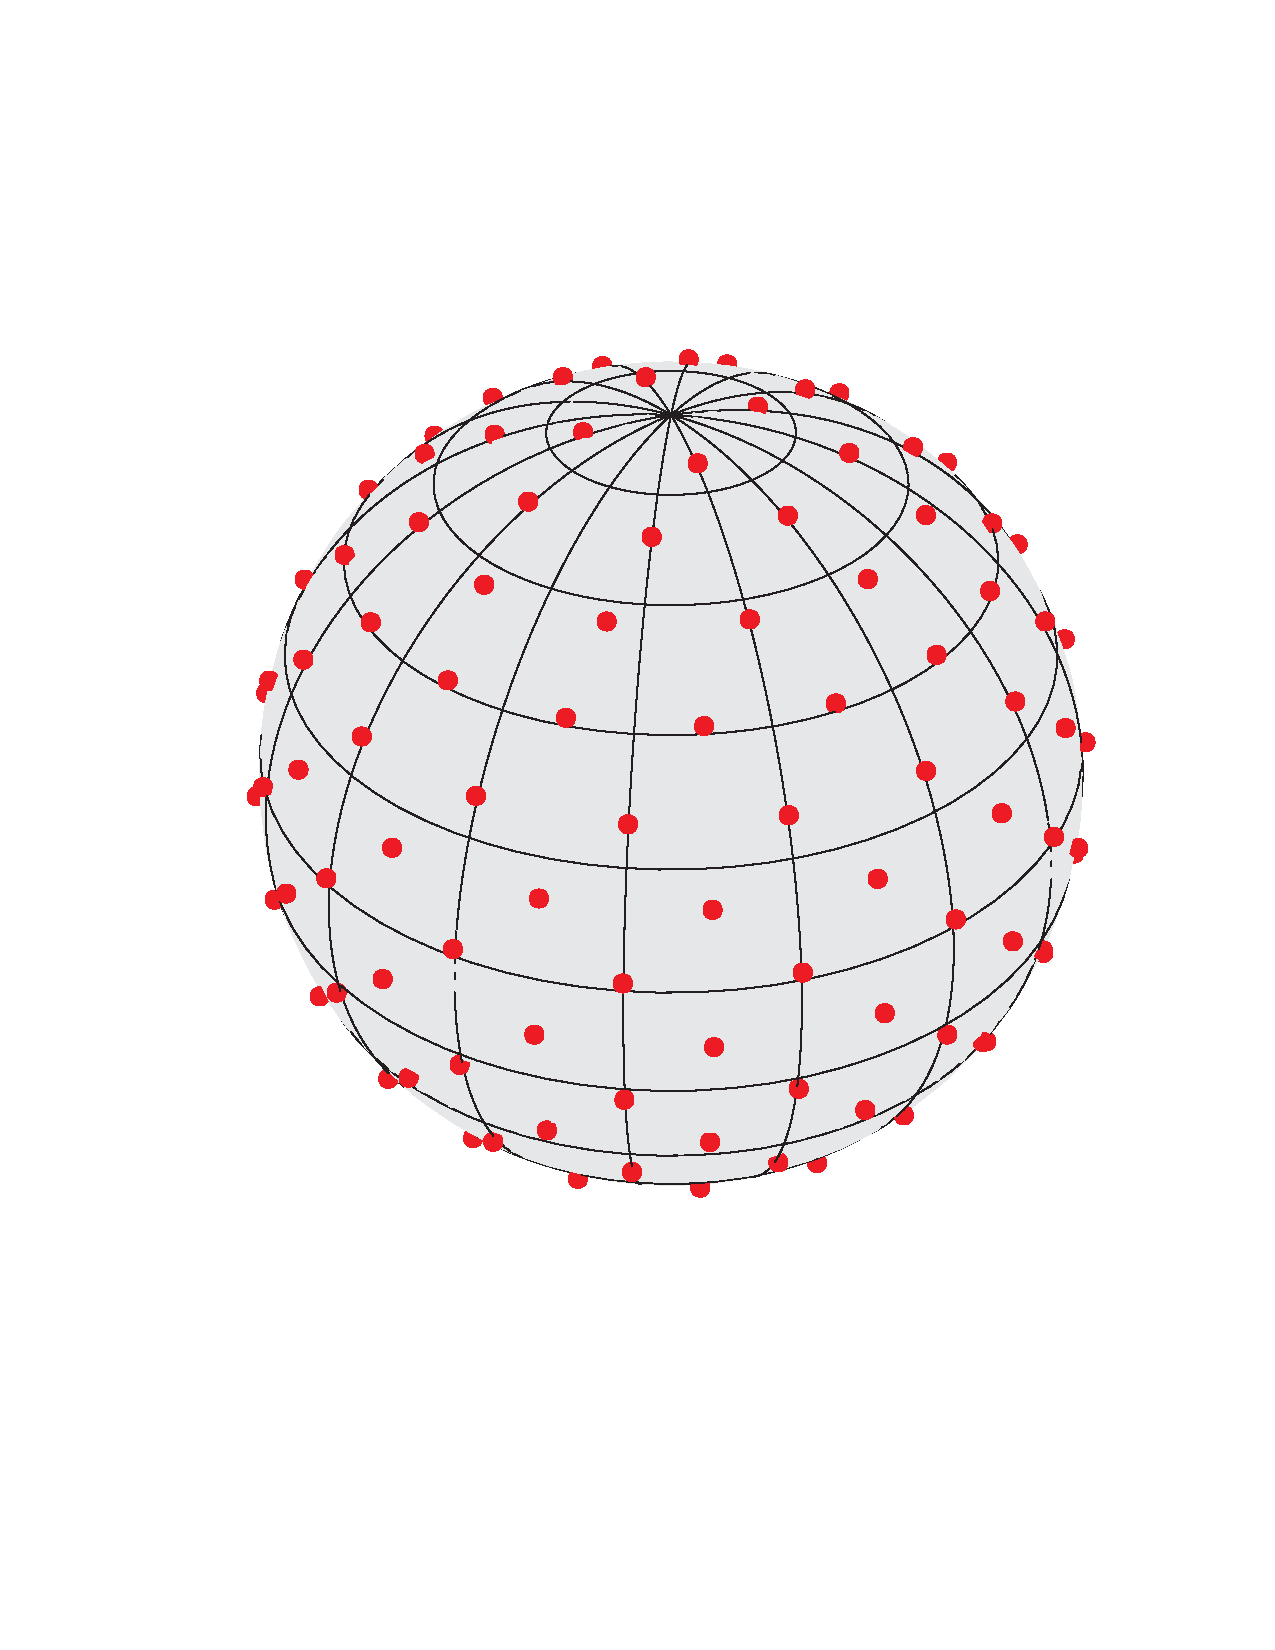
\includegraphics[width=12cm]{images/healpix}
  \caption{To be written...}
  \label{healpix}
\end{figure}


